\documentclass[../../index.tex]{subfiles}

\begin{document}
\chapter{Introduction}
In particle physics we are concerned about small objects and their interactions.
Their dynamics are currently best described by the Standard Model (SM).

The SM contains two groups of fermionic, Spin 1/2 particles. The former group,
the Leptons consist of: the electron ($e$), the muon ($\mu$), the tau ($\tau$)
and their corresponding neutrinos $\nu_e$, $\nu_\mu$ and $\nu_\tau$. The latter
group, the Quarks contain: $u$, $d$ (up and down, the so called light quarks ),
$s$ (strange), $c$ (charm), $b$ (beauty or beauty) and $t$ (top or truth). The SM
furthermore differenciates between three fundamental forces (and its carriers):
the electromagnetic ($\gamma$ photon), weak ($Z$- or $W$-Boson) and strong ($g$
gluon) interactions. The before mentioned Leptons solely interact through the
electromagnetic and the weak force (also refered to as electroweak interaction),
whereas the quarks additionally interact through the strong force.

The strong force is denominated Quantumchromodynamics
(QCD). As the name suggest\footnote{Chromo is the greek word for color.} the
force is characterized by the color charge. Every quark has next to its type one
of the three colors blue, red or green. The color force is mediated through
eight gluons, which each being bi-colored\footnote{Each gluon carries a color
  and an anti-color.}, interact with quarks and each other. The strength of the
strong force is given by the coupling constant $\alpha_s$. The coupling
constants are a function of energy $E$ and $\alpha_s(E)$ increases with 
energy\footnote{In contrast to the electromagnetic force, where $\alpha(E)$
  decreases!}. This is exclusive for QCD and leads to \textit{asymptotic freedom} an
\textit{confinement}. The former phenomen describes the decreasing strong force
between quarks and gluons, which become asymptotically free at large
energies. The latter expresses the fact, that no isolated quark has been found
until today. Quarks appear confined as \textit{Hadrons}, the so called
\textit{Mesons}\footnote{Composite of a quark and an anti-quark.} and
\textit{Baryons}\footnote{Composite of three quarks or three anti-quarks.}.
As we measure \textit{Hadrons} in our experiments but calculate with quarks
within our theoretical QCD model we have to assume \textit{Quark-Hadron
  Duality}, which states that QCD is still valid for Hadrons for energies
sufficently heigh energies. There exist \textit{Duality Violations} (DV), which
will be investigated within this work.

In the following (\cref{sec:tauDecays}) we will describe the $\tau$-decays, which
play an essential role in our QCD analysis. Then (\cref{sec:quantumchromodynamics}) we want to explain some more
details of QCD, especially about the coupling constant $\alpha_s(s)$ (which is not
constant at all) and the \textit{QCD sum rules}.


\section{$\tau$-Decays}
\label{sec:tauDecays}
The $\tau$-particle is an elementary particle with negative electric charge and a
spin of 1/2. Together with the lighter electron and muon it forms the
\textit{charged Leptons}\footnote{Leptons do not interact via the strong force.}.
Even though it is an elementary particle it decays via the \textit{weak
  interaction} with a lifetime of $\tau_\tau=\SI{2.9e-13}{\second}$ and a mass
of $\SI{1776.86\pm0.12}{\mega\electronvolt}$\cite{PDG2018}. It is the only
lepton massive enough to decay into Hadrons.
The final states of a decay are limited by \textit{conservation laws}. In case
of a $\tau$-decay they must conserve the electric charge ($-1$) and
\textit{invariant mass} of the system. Thus, as we can see from
the corresponding Feynman diagram
(see \cref{fig:tauDecay})\footnote{The $\tau$-particle can also decay into strange
  quarks or charm quarks, but these decays are rather uncommon due to the heavy
  masses of s and c.} the $\tau$ decays by the emission of a $\textit{W boson}$
and a tau-neutrino $\nu_\tau$ into different pairs of $(e^-, \bar\nu_e), (\mu^-,
\bar\nu_\mu)$ or $(q, \bar q)$.
\begin{figure}[h]
  \label{fig:tauDecay}
  \centering
  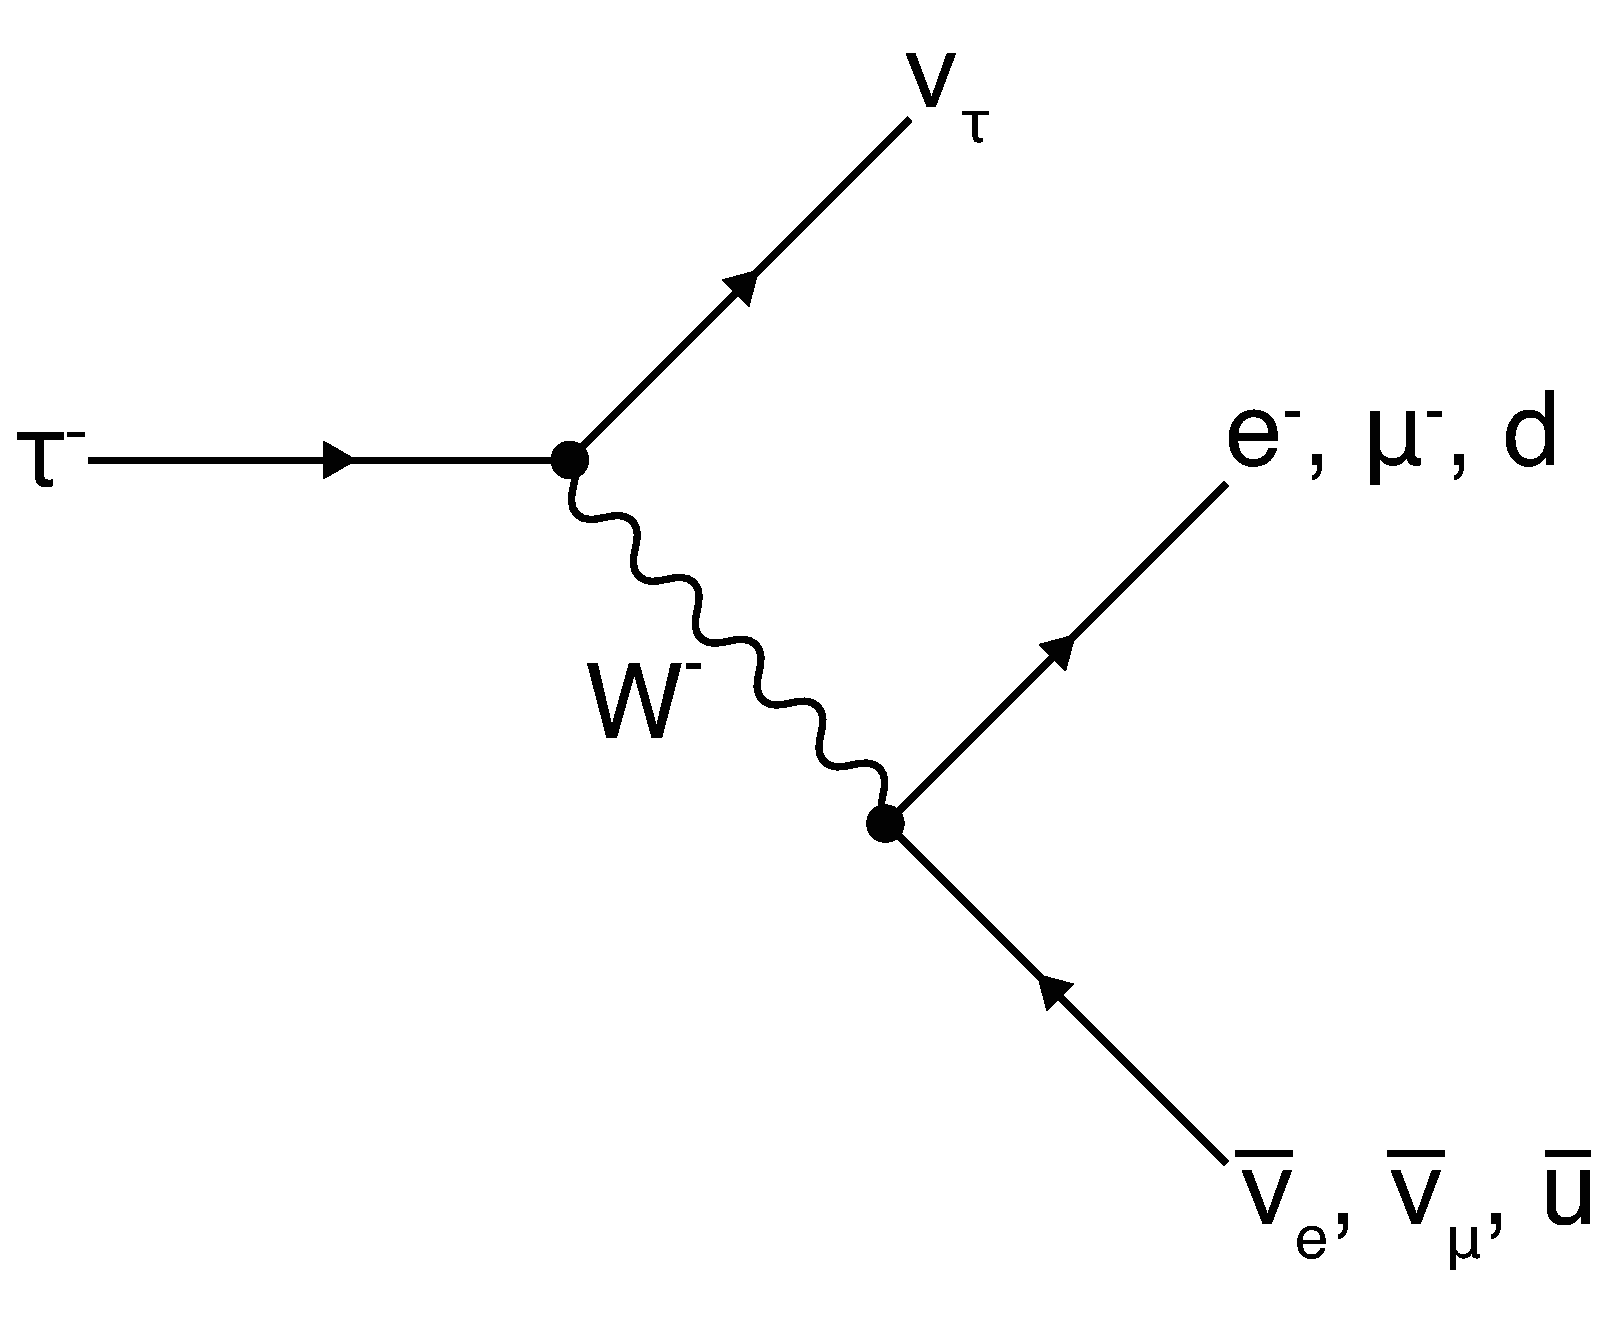
\includegraphics[width=0.4\textwidth]{images/tauDecay.eps}
  \caption{Feynman diagram of common decay of a $\tau$-lepton into pairs of
    lepton-antineutrino or quark-antiquark by the emission of a \textit{W boson}.}
\end{figure}

We are foremost interested into the hadronic decay channels, meaning
$\tau$-decays that have quarks in their final states. Unfortunately the quarks
have never been measured isolated, but appear always in combination of \textit{mesons}
and \textit{baryons}. Due to its mass of $m_\tau \approx
\SI{1.8}{\giga\electronvolt}$ the $\tau$-particle decays into light mesons
(pions-$\pi$, kaons-$K$, and eta-$\eta$, see \cref{table:lightMesons}), which
can be experimentally detected.
\begin{table}
  \label{table:lightMesons}
  \centering
  \begin{tabular}{l c c c}
    \toprule
    Name & Symbol & Quark content & Rest mass ($\SI{}{\mega\electronvolt}$) \\
    \midrule
    Pion & $\pi^-$ & $\bar u d$ & \SI{139.57061 \pm 0.00024}{\mega\electronvolt}  \\
    Pion & $\pi^0$ & $(u \bar u - d \bar d)/\sqrt{2}$ & \SI{134.9770\pm0.0005}{\mega\electronvolt} \\
    Kaon & $K^-$ & $\bar u s$ & \SI{493.677\pm0.016}{\mega\electronvolt} \\
    Kaon & $K^0$ & $d \bar s$ & \SI{497.611\pm0.013}{\mega\electronvolt} \\
    Eta & $\eta$ & $(u \bar u + d \bar d - 2 s \bar s)/\sqrt{6}$ & \SI{547.862\pm0.017}{\mega\electronvolt} \\
  \end{tabular}
  \caption{List of mesons produced by a $\tau$-decay. Rare final states with
    branching Ratios smaller than 0.1 have been omitted. The list is taken from 
    \cite{Davier2006} with corresponding rest masses taken from \cite{PDG2018}.}
\end{table}

The hadronic $\tau-decay$ provides one of the most precise ways to determine the
strong coupling \cite{Pich2016} and can be calculated to high precision within
the framework of QCD.


\section{Quantumchromodynamics}
\label{sec:quantumchromodynamics}
QCD describes the strong interaction, which occur between \textit{quarks} and
are transmitted through \textit{gluons}. A list of quarks can be found in
\ref{table:quarkList}.
\begin{table}
  \label{table:quarkList}
  \centering
  \begin{tabular}{l l c}
    \toprule
    Flavour & Mass & comment\\
    \midrule
    $u$ & $2.2_{-0.4}^{+0.5}$ \SI{}{\mega\eV} & $\overline{\text{MS}}$ \\
    $d$ & $4.7_{-0.3}^{+0.5}$ \SI{}{\mega\eV} \\
    $s$ & $95_{-3}^{+9}$ \SI{}{\mega\eV}  \\
    $c$ & $1.275_{-0.035}^{+0.025}$ \SI{}{\giga\eV} \\
    $b$ & $4.18_{-0.03}^{+0.04}$ \SI{}{\giga\eV} \\
    $t$ & \SI{173.0 \pm 4}{\giga\eV} \\
    \bottomrule 
  \end{tabular}
  \caption{List of Quarks and their masses\cite{PDG2018}.}
\end{table}

The QCD Lagrange density is similar to that of QED\cite{Jamin2006},
\begin{equation}
  \label{eq:qcdLagrangian}
  \mathcal{L}_{QCD}(x) = -\frac{1}{4}G_{\mu\nu}^a(x)G^{\mu\nu a}(x) + \sum_A \left[ \frac{i}{2} \bar{q}^A(x) \gamma^\mu \overleftrightarrow{D}_\mu q^A(x) - m_A\bar{q}^A(x) a^A(x) \right],
\end{equation}
where $q^A(x)$ represents the quark fields and $G_{\mu\nu}^a$ being the \textit{gluon field strength tensor} given by:
\begin{equation}
  \label{eq:gluonField}
  G_{\mu\nu}^a(x) \equiv \partial_\mu B_\nu^a(x) - \partial_\nu^a(x) + g f^{abc} B_\mu^b(x) B_\nu^c(x),
\end{equation}
where $B_\mu^a$ are the \textit{gluon fields}, given in the \textit{adjoint
  representation} of the SU(3) gauge group with $f^{abc}$ as \textit{structure
  constants}. Furthermore we have used $A, B, \dots = 0, \dots 5$ as flavour indices, $a,
b, \dots = 0, \dots, 8 $ as color indices and $\mu, \nu, \dots = 0, \dots 3$ as lorentz indices.


\subsection{Renormalisation Group}
The perurbations of the QCD Lagrangian \ref{eq:qcdLagrangian} lead to divergencies, which have to be
\textit{renormalized}. There are different aproaches to 'make' these
divergencies finite. The most popular one is \textit{dimensional
  regularisation}.
In \textit{Dimensional regularisation} we expand the four space-time dimensions
to arbitrary dimensions. Consequently the in QCD calculations appearing
$\textit{Feyman integrals}$ have to be continued to $D$-dimensions like
\begin{equation}
  \label{eq:dimRegFeynmanIntegral}
  \mu^{2\epsilon} \int \frac{\dif^D p}{(2\pi)^D}\frac{1}{[p^2-m^2+i0][(q-p)^2=m^2+i0]},
\end{equation}
where we introduced the scale parameter $\mu$ to account for the extra
dimensions and conserve the mass dimension of the non continued integral.

In addition \textit{physical quantities}\footnote{Observables that can be
  measured.} cannot depend on the renormalisation scale $\mu$. Thus examining a \textit{physical quantity} $R(q, a_s, m)$ that depends on the
external momentum q, the renormalised coupling $a_s=\alpha_s/\pi$ and the renormalized quark mass $m$ 
\begin{equation}
  \mu \od{}{\mu}R(q, a_s, m) = \left[ \mu \pd{}{\mu} + \mu \od{m}{\mu} \pd{}{m} \right] R(q, a_s, m) = 0
\end{equation}
we can define the \textit{renormalisation group functions}:
\begin{align}
  \beta(a_s) &\equiv -\mu \od{a_s}{\mu} = \beta_1 a_s^2 + \beta_2 a_s^3 + \dots & \beta-\text{function}
  \label{eq:betaFunction} \\
  \gamma(a_s) &\equiv - \frac{\mu}{m} \od{m}{\mu} = \gamma_1 a_s + \gamma_2 a_s^2 + \dots & \text{anomalous mass dimension}.
  \label{eq:anomalousMassDimension}
\end{align}

\subsubsection{Running gauge coupling}
Regarding the $\beta$-function we notice, that $a_s(\mu)$ is not a constant, but
\textit{runs} by varying the scale $\mu$. Integrating the $\beta$-function yields 
\begin{equation}
  \int_{a_s(\mu_1)}^{a_s(\mu_2)}\frac{\dif a_s}{\beta(a_s)} = - \int_{\mu_1}^{\mu_2} \frac{\dif \mu}{\mu} = \log \frac{\mu_1}{\mu_2}.
\end{equation}
To analytically evaluate the above integral we can approximate the $\beta$-function to first order, with the known
coefficient
\begin{equation}
  \beta_1 = \frac{1}{6}(11 N_c - 2 N_f),
\end{equation}
yielding
\begin{equation}
  a_s(\mu_2) = \frac{a_s(\mu_1)}{\left( 1 - a_s(\mu_1) \beta_1 \log\frac{\mu_1}{\mu_2} \right)}.
\end{equation}
As we have three colours $N_c=3$ and six flavours $N_f=6$ the first
$\beta$-function \ref{eq:betaFunction} is positive. Thus for $\mu_2>\mu_1$ $a_s(\mu_2)$ decreases
logarithmically and vanishes for $\mu_2 \to \infty$. This behaviour is known as
\textit{asymptotic freedom}.
The coefficients of the $\beta$-function are currently known up to the 5th
order, which are displayed in the appendix \ref{sec:betaCoefficients}.

\subsubsection{Running quark mass}
The properties of the running quark mass can be derived similar to the gauge
coupling. Starting from integrating the \textit{anomalous mass dimension} \ref{eq:anomalousMassDimension}
\begin{equation}
  \log \frac{m(\mu_2)}{m(\mu_1)} = \int_{a_s(\mu_1)}^{a_s(\mu_2)} \dif a_s \frac{\gamma(a_s)}{\beta(a_s)}
\end{equation}
we can approximate the \textit{anomalous mass dimension} to first order and
solve the integral analytically \cite{Schwab2002}
\begin{equation}
  m(\mu_2) = m(\mu_1)\left( \frac{a(\mu_2)}{a(\mu_1)} \right)^{\frac{\gamma_1}{\beta_1}} \left( 1 + \mathcal{O}(\beta_2, \gamma_2) \right).
\end{equation}
As $\beta_1$ and $\gamma_1$ (see \ref{app:gammaCoefficients}) are positive the
quark mass decreases with increasing $\mu$.
The general relation between different scales is given by
\begin{equation}
  m(\mu_2) = m(\mu_1) \exp \left( \int_{a_s(\mu_1)}^{a_s(\mu_2)} \dif a_s \frac{\gamma(a_s)}{\beta(a_s)}  \right)
\end{equation}
and can be solved numerically to run the quark mass to the needed scale $\mu_2$.

\subsection{Sum Rules}
We need to relate the measurable hadronic final states of a QCD process (e.g.
$\tau$-decays into Hadrons) to a theoretical calculable value. Consequently we will employ \textbf{QCD Sum Rules}\cite{Shifman1978}, which is a combination of the \textbf{operator
  product expansion} (OPE), the \textbf{optical theorem}, a \textbf{dispersion
relation} the analyticity of the \textbf{two-poin function} and the \textbf{quark
hadron duality}. 

Starting from the the vacuum expectation value of the product of the conserved
noether current $J_\mu(x)$ at different space-times points $x$ and $y$, which
is known as the
\textit{two-point function} (or simply correlator)
\begin{equation}
  \label{eq:twoPointFunction}
  \Pi(q^2) = \langle  0 | J_\mu(x) J_\nu(y) | 0 \rangle,
\end{equation}
where the noether current is given by
\begin{equation}
  J_\mu(x) = \Psi^\dagger(x) \gamma_\mu (\gamma_5) \Psi(x).
\end{equation}
The two-point function, within the framework of QCD sum rules, is improved by
the OPE expansion
\begin{equation}
  \Pi_{OPE}(s) = \sum_n C_{2n}(s, \mu) \frac{\langle \hat{\mathcal{O}} (\mu) \rangle }{s^{n}},
\end{equation}
where we used $q^2=s$. It is furthermore related to the hadronic
\textbf{spectral function} $\rho(q^2)$ through the \textit{Källén-Lehmann
  spectral representation} \cite{Kallen1952}\cite{Lehmann1954}
\begin{equation}
  \label{eq:dispersionRelation}
  \Pi(q^2) = \int_0^\infty \dif s \frac{\rho(s)}{s - q^2 - i \epsilon},
\end{equation}
where the spectral function $\rho(s)$ is defined as
\begin{equation}
  \rho(s) \equiv \frac{1}{\pi} \Ima \Pi(s).
\end{equation}
Equation \ref{eq:dispersionRelation} is refered to as \textbf{dispersion relation} analogous to similar
realtions which arise for example in electrodynamics.
The the main contribution from the spectral function given in
\cref{eq:dispersionRelation} are the hadronic final states
\begin{equation}
  2 \pi \rho(m^2) = \sum_n \langle  0 | J_\mu(x) | n \rangle \langle n | J_\nu(y) \rangle (2 \pi^2)^4 \delta^{(4)}(p - p_n),
\end{equation}
which lead to a series of continuos poles on the positive real axis for the
two-point function, see Fig. \ref{fig:analyticStructureCorrelator}.
\begin{figure}[h]
  \centering
  \label{fig:analyticStructureCorrelator}
  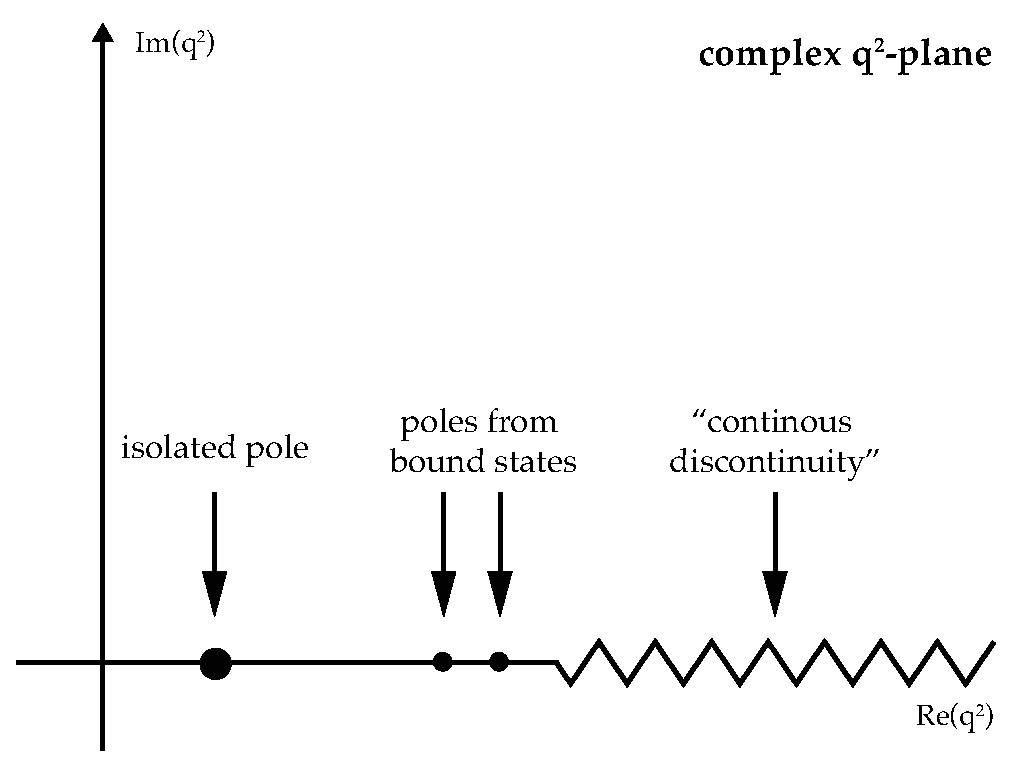
\includegraphics[width=0.8\textwidth]{./images/analyticStructureCorrelator.eps}
  \caption{Analytic structure in the complex $q^2$-plane of the Fourier
    transform of the two-point function. The hadronic final states are
    responsible for poles appearing on the real-axis. The one-particle states contribute as
    isolated pole and the multi-particle states contribute as bound-states poles
    or a continues ``discontinuity cut'' (see \cite{Peskin1995}).}
\end{figure}
As the experimental data, which solely contributes to the spectral function
$\rho(q^2)$, is only accesible on the postive real axis, we have to use Cauchy's
theorem to access the theoretical values of the two-point function close to the
postive real axis (see \cref{fig:correlatorComplexContour}).
\begin{figure}[h]
  \centering
  \label{fig:correlatorComplexContour}
  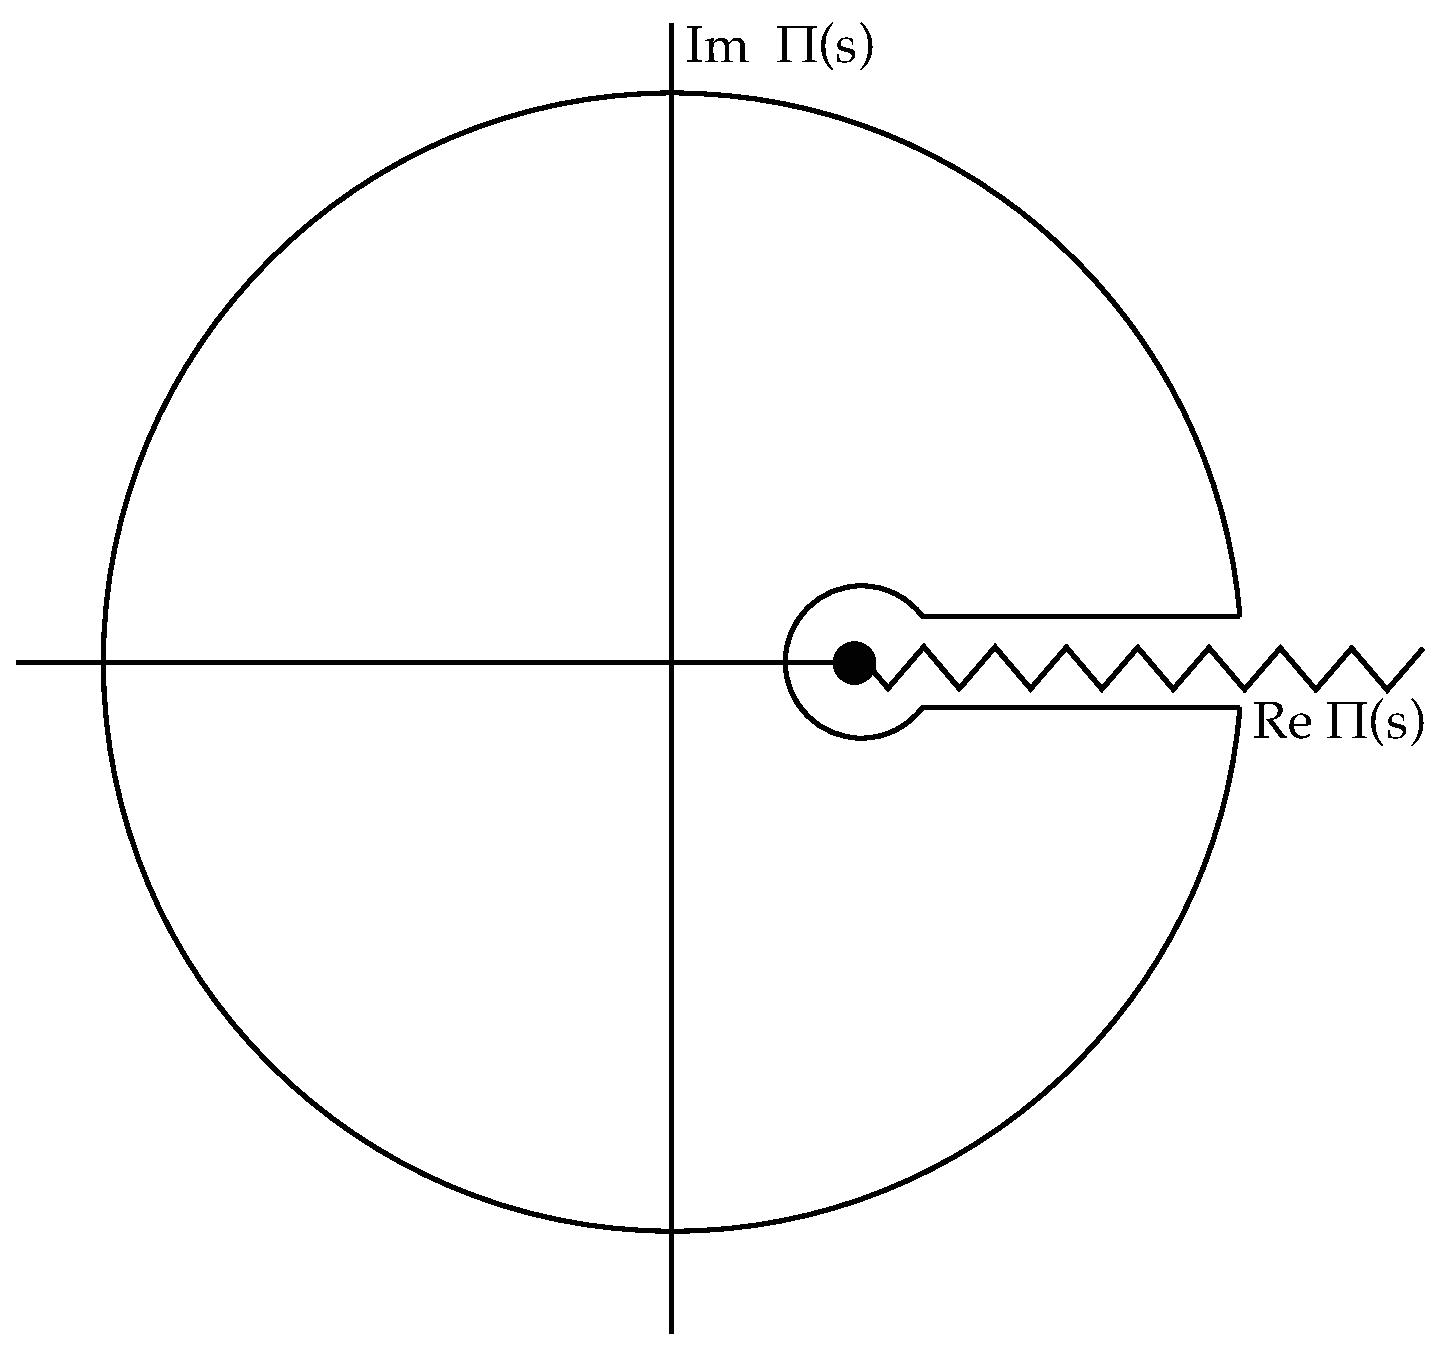
\includegraphics[width=0.6\textwidth]{./images/correlatorComplexContour.eps}
  \caption{Analytical structure of $\Pi(s)$ with the used contour $\mathcal{C}$
    for the final QCD Sum Rule expression \cref{eq:qcdSumRules}.}
\end{figure}

The final ingredient of the QCD sum rules is the \textit{optical theorem},
relating experimental data with the imaginary part of the correlator. E.g.
taking the the total $e^+ e^-$ cross section scattering into hadrons
\begin{equation}
  R_q(s) \equiv \frac{\sigma(e^+ e^- \to \gamma^* \to q \bar q)}{\sigma(e^+ e^- \to \mu^+ \mu^-)} = 12 \pi \Ima \Pi_{Had}(s).
\end{equation}
Due to asymptotic freedom\footnote{There are no free quarks. They are bound in
  pairs of two or three.} experiments can only detect Hadrons (note the
$exp$-indice in $\Ima \Pi_{exp}(s)$), but on the theory
side we are calculating with quarks as degrees of freedom. Consequently we
assume that $\Pi_{Had}$ can be set equal to $\Pi_{OPE}$, which is referred
to as \textit{quark hadron duality}.

In total, with the help Cauchy's theorem, the QCD sum rules can be sumed up in
the following expression
\begin{equation}
  \label{eq:qcdSumRules}
  \frac{1}{\pi}\int_0^\infty \frac{\Ima \Pi_{Had}(t)}{t - s}\dif t = \frac{1}{\pi} \oint_{\mathcal{C}} \frac{\Ima \Pi_{OPE}(t)}{t -s}\dif t,
\end{equation}
where the l.h.s. is given by the experiment and the r.h.s. can be theoretically
evaluated with by applying the OPE of the correlator $\Pi_{OPE}(s)$.

\end{document}